\section{Empirical analysis}
\label{sec:experiment}
%-----------------------------------------------------------
\subsection{Datasets description}

Each of the considered progress prediction methods evaluates on different datasets: \textsl{RSDNet} on \textsl{Cholec80} \cite{twinanda2016}, \textsl{ProgressNet} on \textsl{UCF101-24} \cite{soomro2012}, and \textsl{UTE} on \textsl{Breakfast} \cite{kuehne2014, kuehne2016}. 
To analyze these methods, we use all 3 datasets for all methods. 

\smallskip\noindent\textbf{\textsl{Cholec80} \cite{twinanda2016}}: Consists of 80 videos of endoscopic cholecystectomy surgery.  
Note that \cite{twinanda2019} uses an extended version of this dataset, \textsl{Cholec120}, containing 40 additional surgery videos. 
However, \textsl{Cholec120} is not publicly available, so we used \textsl{Cholec80} to report our results. 
We randomly create four folds of the data, and follow the same train\slash test dataset split sizes as in \cite{twinanda2019}. 
This dataset has limited visual variability both across training and test splits.
Moreover, the presence of different medical tools in the frames informs of the different surgery phases, which could aid the progress prediction task.

\smallskip\noindent\textbf{\textsl{UCF101-24} \cite{soomro2012}:} Consists of a subset of \textsl{UCF101} containing 24 activities, each provided with a spatio-temporal action tube annotation.\footnote{Following \cite{becattini2017} we use the revised annotations available at \url{https://github.com/gurkirt/corrected-UCF101-Annots}} 
Becattini \etal \cite{becattini2017} split the dataset into 2 categories: \textsl{telic} and \textsl{atelic} activities.
\textsl{Telic} activities are those with a clear endpoint, such as `cliff diving', while \textsl{atelic} activities, such as `walking the dog', do not have a clearly defined endpoint. 
Predicting progress for \textsl{atelic} activities is more difficult than for \textsl{telic} ones.
The original implementation of \textsl{ProgressNet} first trains on \textsl{telic} activities, and then fine-tunes on all activities. 
We did not observe a difference when using this training procedure, and instead train all methods on the full dataset.

\smallskip\noindent\textbf{\textsl{Breakfast} \cite{kuehne2014, kuehne2016}:} Contains 10 cooking activities: \eg `making coffee', `baking pancakes', or `making tea', etc., performed by 52 individuals in 18 different kitchens. 
We use the default splits and train each model across all cooking activities. 
Because the tasks are performed by different individuals in different kitchens, the video appearance varies even within the same task, making this dataset extra challenging for progress prediction.

\textsl{UCF101-24} contains training videos of up to 599 frames, while \textsl{Cholec80} and \textsl{Breakfast} contain videos with thousands of frames.
When training on \textsl{full-videos}, we could not train the \textsl{ProgressNet} model on the original \textsl{Cholec80} and \textsl{Breakfast} datasets, because of the long videos leading to memory problems.
Thus, for the experiments on \textsl{full-videos}, we use a subsampled version of \textsl{Cholec80} from 1 fps to 0.1 fps (the original fps is 25; \cite{twinanda2019} subsamples this down to 1 fps); and we subsample the \textsl{Breakfast} dataset from 15 fps down to 1 fps. 
For our experiments on \textsl{video-segments} we use the original datasets.

\begin{figure*}
\centering
    \begin{tabular}{ccc}
    \multicolumn{3}{c}{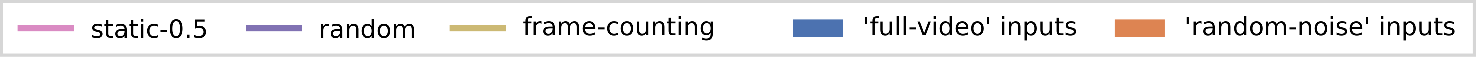
\includegraphics[width=.8\linewidth]{media/results/legend_full2.pdf}} \\
    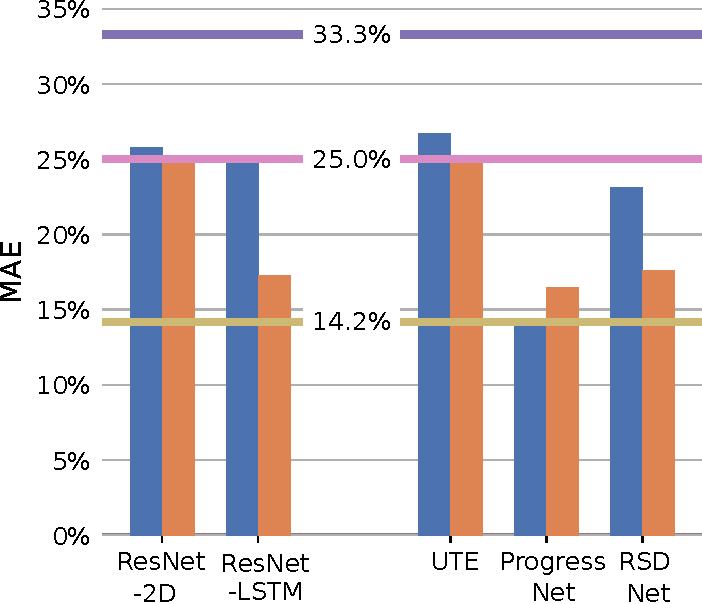
\includegraphics[width=0.31\linewidth]{media/results/ucf_full-1.pdf} & 
    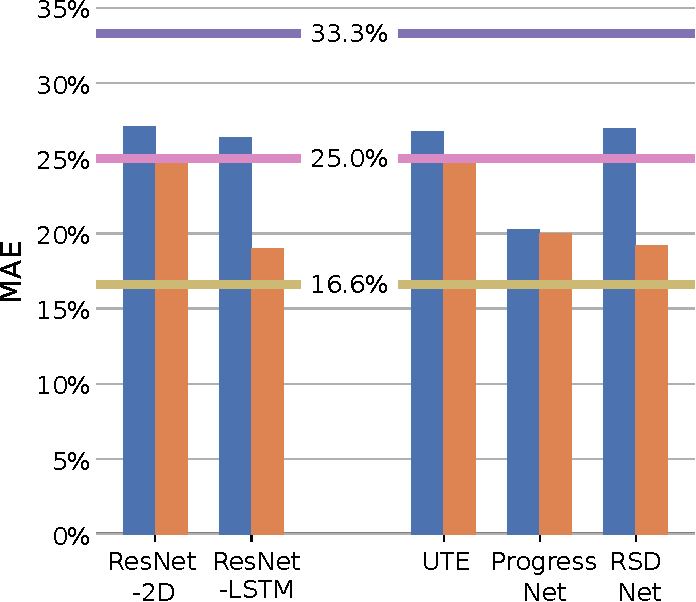
\includegraphics[width=0.31\linewidth]{media/results/breakfast_full-1.pdf} &
    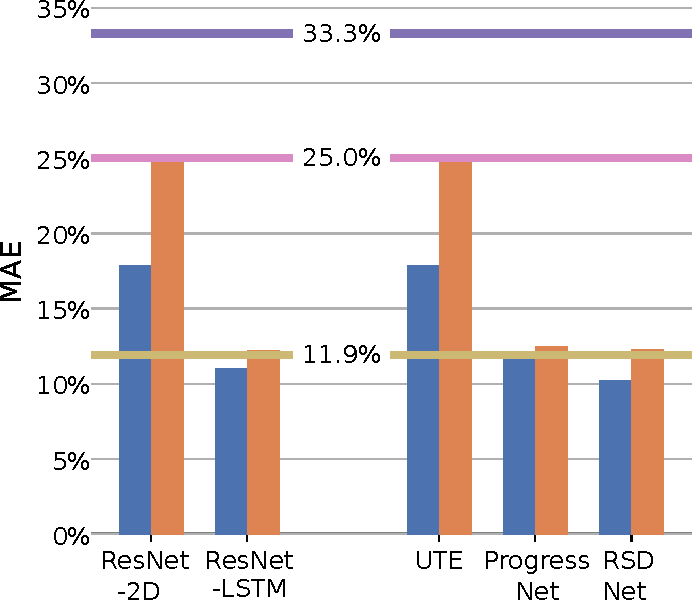
\includegraphics[width=0.31\linewidth]{media/results/cholec_full-1.pdf} \\
    {\small (a) \textsl{UCF101-24} on \textsl{full-videos}.} &
    {\small (b) \textsl{Breakfast} on \textsl{full-videos}.} &
    {\small (c) \textsl{Cholec80} on \textsl{full-videos}.} \\
    \end{tabular}
   \caption{\textbf{MAE scores on \textsl{full-videos}}. 
       We plot the MAE in percentages for all learning methods when inputting both \textsl{full-video} data and \textsl{random-noise}. 
       (a) MAE for the \textsl{UCF101-24} dataset: For all methods except \textsl{ProgressNet} inputting \textsl{random-noise} performs on par or better than inputting \textsl{full-videos}.
       (b) MAE for the \textsl{Breakfast} dataset: When using \textsl{random-noise} as input to the methods, they perform on par or better than when inputting \textsl{full-videos}, indicating that the methods overfit to training artifacts.
       (c) MAE for the \textsl{Cholec80} dataset: On this dataset, using visual \textsl{full-videos} is better than inputting \textsl{random-noise}, however the \textsl{frame-counting} baseline remains hard to exceed.
   }
\label{fig:full}
\end{figure*}
%-----------------------------------------------------
%-----------------------------------------------------
%-----------------------------------------------------
\subsection{Experimental setup}
For the considered progress prediction methods only the code for \textsl{UTE} is published.\footnote{\url{https://github.com/Annusha/unsup_temp_embed}} 
For the other methods, we follow the papers for implementation details and training procedures. 
We train \textsl{RSDNet} in a 2-step procedure following \cite{twinanda2019}, however for training the LSTM blocks we found that using the Adam optimizer with a learning rate of $10^{-4}$ and no weight decay, for $30$k iterations works best. 
For \textsl{ProgressNet} not all training details are mentioned in the paper, so we use Adam with a learning rate of $10^{-4}$ for $50$k iterations, and we keep the VGG-16 backbone frozen during training. 
For all experiments we report the MAE (Mean Absolute Error) in percentages.
Our code is available online at \href{https://github.com/Frans-db/progress-prediction}{https://github.com/Frans-db/progress-prediction}.

%-----------------------------------------------------
%-----------------------------------------------------
%-----------------------------------------------------
\subsection{\textbf{\emph{(i) How well can methods predict activity progression on the current datasets?}}}
\noindent\textbf{(i.1) Progress predictions on \textsl{full-videos}.}
Here we want to test how well the learning-based models perform when trained on \textsl{full-videos}.
We compare this with using \textsl{random-noise} as input -- we replace each frame with randomly sampled noise. 
Intuitively, learning from \textsl{random-noise} over complete videos will give recurrent models access to frame indices, and this should reach the \textsl{frame-counting} baseline, which computes dataset statistics per frame.
If the models learn to extract useful appearance information, their MAE scores should be considerably higher than when inputting \textsl{random-noise}.
Additionally, we compare the learning-based methods with the naive baselines: \textsl{static-0.5}, \textsl{random}, and \textsl{frame-counting}.

\fig{full}(a) shows that the \textsl{full-video} visual information (blue bars) is less useful than inputting \textsl{random-noise} (orange bars).
When training on the \textsl{full-videos} of \textsl{UCF101-24} both the \textsl{ResNet-2D} and \textsl{UTE} models perform on par with the \textsl{static-0.5} baseline.
This is because these spatial-only networks do not have any way of integrating temporal information and they fail to extract progress information from the visual data alone.
When provided with \textsl{random-noise} as inputs, they always predict $0.5$ and score on par with the \textsl{static-0.5} baseline. 
The results are similar for the recurrent models on \textsl{full-videos}, \textsl{ResNet-LSTM} and \textsl{RSDNet} who are both close to the \textsl{static-0.5} baseline. 
We observe that the recurrent models overfit on the embedded features and fail to generalise. 
When these recurrent networks are provided with \textsl{random-noise} they can only rely on the number of frames seen so far, and thus reach the \textsl{frame-counting} baseline. 
\textsl{ProgressNet} is the only outlier here: when given \textsl{full-videos} it performs better than when given \textsl{random-noise} as input. 
However, \textsl{ProgressNet} still cannot outperform the non-learning \textsl{frame-counting} baseline.

For \textsl{Breakfast} in \fig{full}(b) the results look very similar to those on \textsl{UCF101-24}. 
Both the \textsl{ResNet-2D} and \textsl{UTE} models cannot learn from visual information alone. \textsl{ResNet-LSTM} and \textsl{RSDNet} both perform worse than the \textsl{static-0.5} baseline on \textsl{full-videos}, indicating that they are overfitting on the training data. 
When provided with \textsl{random-noise} as input, they again can only rely on the number of frames seen, and thus approach the \textsl{frame-counting} naive baseline. 

\textsl{Cholec80} in \fig{full}(c) is the only dataset where the spatial-only networks \textsl{ResNet-2D} and \textsl{UTE} perform better than the \textsl{static-0.5} baseline.
Here, we see that using the \textsl{full-videos} (blue bars) is better than inputting \textsl{random-noise} (orange bars).
This hints to the visual information present in this dataset being indicative of the activity progress. 
When inputting \textsl{random-noise} the spatial-only methods again perform on par with the \textsl{static-0.5} baseline, as expected. 
However, this dataset still remains challenging as the methods are not far from the \textsl{frame-counting} baseline.
\textsl{ResNet-LSTM} and \textsl{RSDNet} are the only who perform slightly better than this naive baseline, indicating that they can extract some useful visual information from the video frames. 

\smallskip\noindent\textbf{Observation:} 
\emph{
The current datasets make it difficult for the progress prediction methods to extract useful visual information.
Therefore, the methods overfit to training set artifacts, and are outperformed by simple baselines based on dataset statistics.}

\begin{figure*}
\centering
    \begin{tabular}{ccc}
    \multicolumn{3}{c}{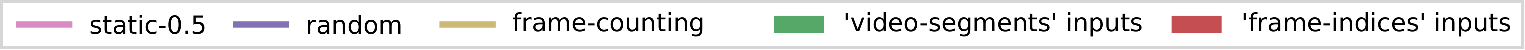
\includegraphics[width=.8\linewidth]{media/results/legend_seg2.pdf}} \\
    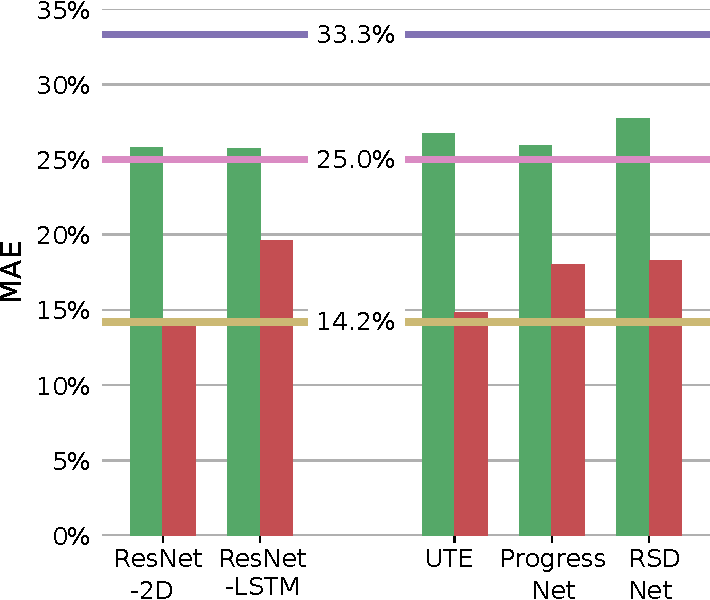
\includegraphics[width=0.31\linewidth]{media/results/ucf_seg.pdf} & 
    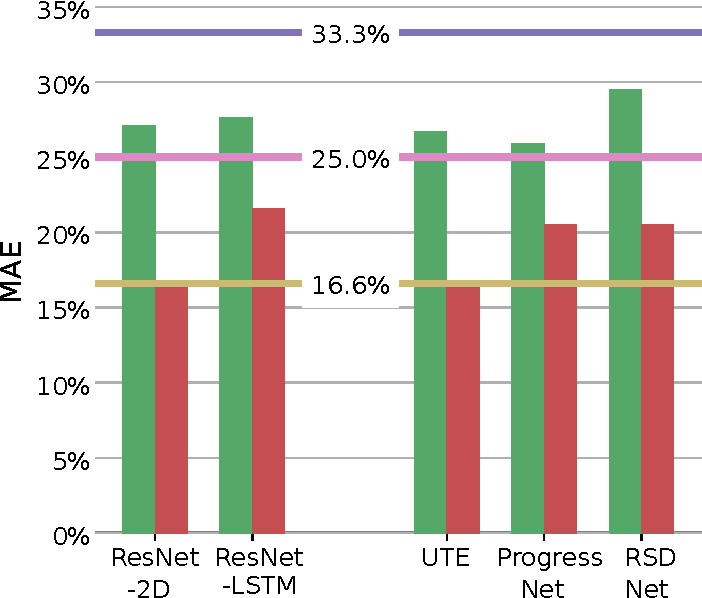
\includegraphics[width=0.31\linewidth]{media/results/breakfast_seg.pdf} &
    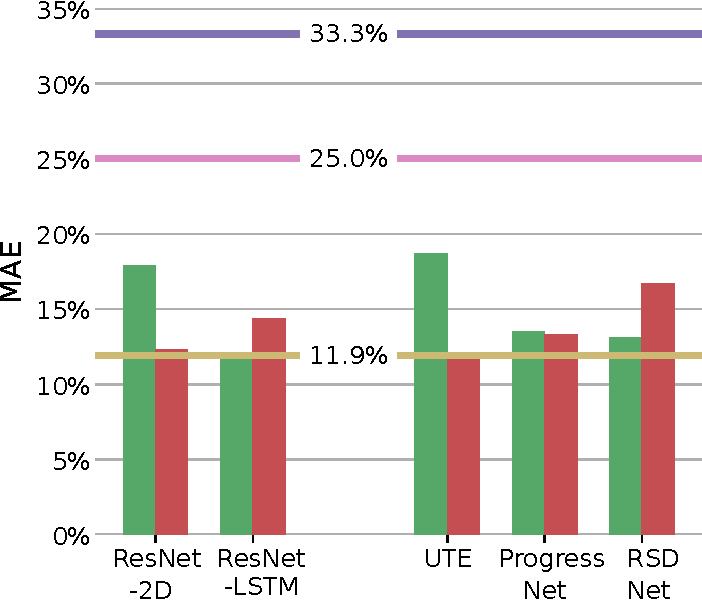
\includegraphics[width=0.31\linewidth]{media/results/cholec_seg.pdf} \\
    {\small (a) \textsl{UCF101-24} on \textsl{video-segments}.} &
    {\small (b) \textsl{Breakfast} on \textsl{video-segments}.} &
    {\small (c) \textsl{Cholec80} on \textsl{video-segments}.} \\
    \end{tabular}
   \caption{\textbf{MAE scores on \textsl{video-segments}}. 
       We plot the MAE in percentages for all considered methods when inputting both \textsl{video-segments} and \textsl{frame-indices}. 
       (a) MAE for the \textsl{UCF101-24} dataset: For all methods inputting \textsl{frame-indices} is better than inputting \textsl{video-segments}. 
        \textsl{ResNet-2D} and \textsl{UTE} get the biggest boost in performance because they can learn the one-to-one mapping from index to progress during training. 
       (b) MAE for the \textsl{Breakfast} dataset: Also here \textsl{frame-indices} are more informative than the visual data.
       (c) MAE for the \textsl{Cholec80} dataset: All learning methods perform on par with the \textsl{frame-counting} baseline, except for \textsl{RSDNet} which is slightly worse. 
        This could be due to suboptimal hyperparameter settings. 
   }
\label{fig:seg}
\end{figure*}
%-----------------------------------------------------------------------------------
\medskip\noindent\textbf{(i.2): Progress predictions on \textsl{video-segments}.}
We test the performance of learning methods when trained to predict progress from \textsl{video-segments}.
Using \textsl{video-segments} should encourage the methods to focus more on the visual information and not on the temporal position of the frames, as this is no longer informative. 
We compare inputting \textsl{video-segments} with inputting \textsl{frame-indices} -- the absolute index of each frame, replicated as images.
Intuitively, learning from \textsl{frame-indices} should be on par with the \textsl{frame-counting} baseline, since the only information available is the dataset statistics per frame.
Ideally, we would expect all methods to solve the progress prediction task by relying on visual information, and therefore having lower errors than when inputting \textsl{frame-indices}.
Again, we also compare with the naive baselines: \textsl{static-0.5}, \textsl{random} and \textsl{frame-counting}. 

\fig{seg}(a) shows that the visual information encoded in \textsl{video-segments} (green bars) is less useful than knowing the current frame index (red bars).
When trained on \textsl{video-segments} of \textsl{UCF101-24} all methods perform on par with the \textsl{static-0.5} baseline.
Thus, the models cannot learn to predict progress from the visual video data. 
Interestingly, \textsl{ProgressNet} using \textsl{full-videos} in \fig{full}(a) is better than the \textsl{frame-counting} baseline, however, here it fails to learn when trained on \textsl{video-segments}. 
When provided with \textsl{frame-indices} as input, all methods improve. 
The improvement is most visible for \textsl{ResNet-2D} and \textsl{UTE}, which do not use recurrent blocks. 
This is because the non-recurrent methods can learn the one-to-one mapping from index to progress during training. 

The results on the \textsl{Breakfast} dataset in \fig{seg}(b) are similar to those of \textsl{UCF101-24} in \fig{seg}(a). 
None of the networks can extract useful information from the \textsl{video-segments}.
All methods improve when trained on \textsl{frame-indices}.
The improvement is again more obvious for \textsl{ResNet-2D} and \textsl{UTE}.
Moreover, all results are on par with, or worse than the \textsl{frame-counting} baseline. 

On \textsl{Cholec80} in \fig{seg}(c) all results are close to the \textsl{frame-counting} baseline. 
This is dissimilar to \fig{full}(c) where inputting visual data was better than inputting random noise of the same length as the full video.
Again, \textsl{ResNet-2D} and \textsl{UTE} improve when provided with \textsl{frame-indices} as input. 
For \textsl{ResNet-LSTM} and \textsl{ProgressNet} and \textsl{RSDNet} the performance is on par with the \textsl{frame-counting} baseline when trained on \textsl{video-sequences} indicating that these methods overfit to the training data.
When trained on \textsl{frame-indices} most methods approach the \textsl{frame-counting} baseline, as this is the information encoded in the frame indices across the full training set.
\textsl{RSDNet} performs worst when given \textsl{frame-indices} as inputs;  we hypothesise that this is due suboptimal hyperparameter settings. 

\smallskip\noindent\textbf{Observation:} 
\emph{
When restricting the models to rely only on visual information, the models are outperformed by simply considering the current frame index, and performing dataset statistics.
This is due to the current progress prediction datasets not containing sufficient visual information to guide progress prediction.}


%-------------------------------------------------------------------------------
\subsection{\emph{\textbf{(ii) Is it at all possible to predict activity progress from visual data only?}}}
We observe that current progress prediction datasets are not well-suited for the task, as the learning models fail to extract useful information from visual data alone. 
To test that the problem is indeed with the datasets used for evaluation and not the learning models, we test here if progress prediction is possible from visual data alone.
For this we aim to construct a synthetic dataset in such a way that the learning-based methods perform optimal using visual information, and outperform all the naive baselines.

Our synthetic \textsl{Progress-bar} dataset, shown in \fig{progressbars}, contains a progress bar (similar, for example, to a download bar) that slowly fills up from left to right. 
Each frame has a resolution of $32{\times}32$px. 
We generate $900$ videos for the training split, and $100$ for the test split.
Each bar has its own rate of progression, but there is a variance per notch causing some uncertainty. 
Therefore, even on this simple dataset it is impossible to make no errors.
This is why in the first image the progression appears to be slightly beyond 25\%, but because the video may slow down after this section it is actually at 22.2\%. 
Due to the large variance in video length, ranging from $19$ to $145$ frames, the \textsl{frame-counting} baseline, and thus frame-counting strategies, will give worse results than relying on visual information.
Also, because of the different progress rates per video, the learning methods cannot just rely on visual information alone, but also have to use temporal information to perform well on this progress prediction task. 
\begin{figure}[t]
\begin{center}
   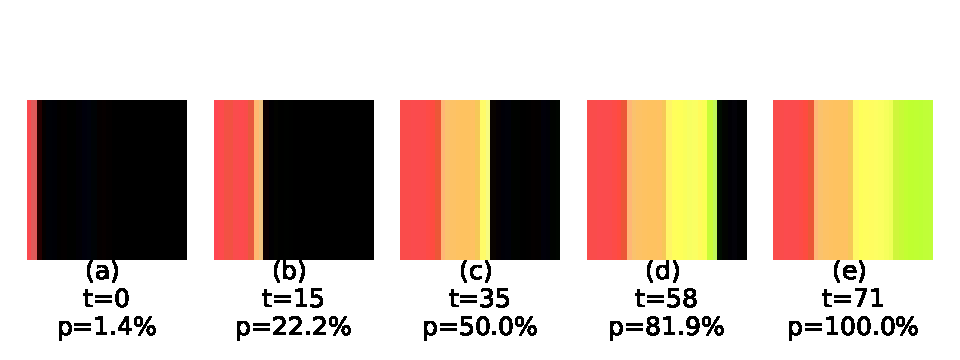
\includegraphics[width=1.0\linewidth]{media/bars.pdf}
\end{center}
   \caption{Visualisation of a progress bar from our synthetic \textsl{Progress-bar} dataset at timesteps $t{=}0$, $t{=}15$, $t{=}35$, $t{=}58$, and $t{=}71$. 
   Each coloured section indicates visually a 25\% section, but due to variance in the speed, the actual video progress may differ at these points.
   }
\label{fig:progressbars}
\end{figure}
Due to the reduced frame resolution and data complexity of our synthetic dataset, we scale down the \textsl{ResNet} backbone, for these experiments. 
Specifically, to avoid overfitting, we use \textsl{ResNet-18} as a backbone for \textsl{ResNet-2D}, \textsl{ResNet-LSTM}, and \textsl{RSDNet}. 
\textsl{ProgressNet} and \textsl{UTE} remain unchanged.


\fig{result_bars} shows the results of all the learning-based methods when predicting progress from both \textsl{full-videos} and \textsl{video-segments}. 
For this dataset the \textsl{frame-counting} baseline has an MAE of $12.9$\%, which is outperformed by all learning-based methods. 
\textsl{UTE} performs the best out of all the networks, even though it does not have memory. 
This is because \textsl{UTE} relies on 3D convolutional embeddings over a temporal-window of size $16$ frames. 
This temporal-window gives the method information about $7$ future frames, which is sufficient on this simple dataset. 
For the LSTM-based methods inputting \textsl{full-videos} still performs slightly better than inputting \textsl{video-segments}. 
At a closer look, this is because the \textsl{video-segments} sampling method has a bias towards frames in the middle of a video. 
The earlier frames are less likely to get sampled, thus the progress prediction methods will have a higher error there.

\smallskip\noindent\textbf{Observation:} 
\emph{It is feasible for the progress prediction methods to make effective use of the visual data present in the videos and outperform the \textsl{frame-counting} baseline, when the visual data is a clear indicator for the video progression.
}
\begin{figure}
\begin{center}
   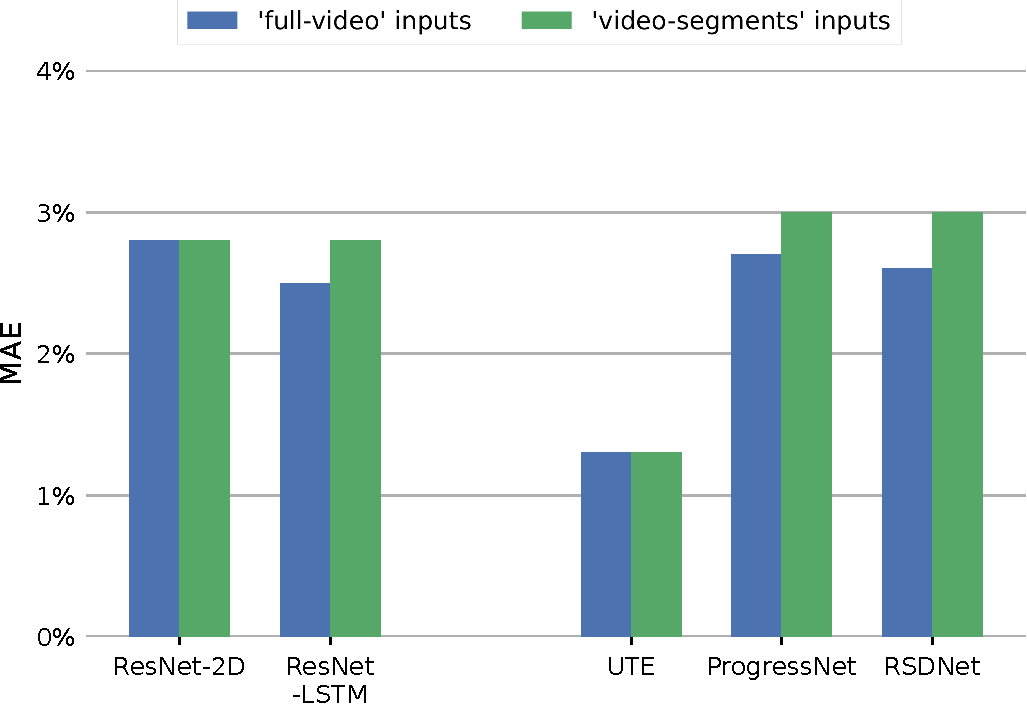
\includegraphics[width=1.0\linewidth]{media/results/bars.pdf}
\end{center}
   \caption{\textbf{MAE scores on our synthetic \textsl{Progress-bar} dataset, when training on \textsl{full-videos} and \textsl{video-segments}}. 
   The \textsl{frame-counting} baseline has an MAE of $12.9\%$, while the \textsl{static} baseline is at $25\%$ and the \textsl{random} baseline at $33.3\%$. 
   We see that all methods outperform the \textsl{frame-counting} baseline. 
   \textsl{UTE} obtains the best result due to its $15$-frame temporal window, which allows it to see $7$ frames into the future. 
   We conclude that the progress prediction methods are able to learn progress from visual information, if it is clearly present in the videos.}
\label{fig:result_bars}
\end{figure}